%preamble
\documentclass[letterpaper]{article}
\synctex=1
\usepackage{graphicx}
\graphicspath{ {images/} }

\usepackage{lipsum}
\usepackage{float}
% \bibliographystyle{IEEEtran}
\bibliographystyle{ieeetr}

\usepackage{amssymb}

\usepackage{siunitx}
%actual document
\begin{document}

  % \maketitle %insert titlepage here
  \begin{titlepage}
    \begin{center}
        \vspace*{1cm}
        \Huge
        Experiment 4
        \vspace{1cm}

        Magnetic Fields
        \vspace{1cm}

        By: Arun Woosaree
        \vspace{1cm}

        Lab partners:
        \vspace{.25cm}
        \Large

        Fatemeh Ghafari Far\\
        % Purvish Jajal
        \vspace{.25cm}
        Yvonne Hong
        \vspace{1cm}

        \Huge
        PHYS 230 Lab EH71
        \vspace{1cm}

        TA: Andrei Tretiakov
        \vspace{1cm}

        Date of Lab: March 22, 2018%\today
        \vfill
    \end{center}
\end{titlepage}

\section{Introduction}
% Begin with experiment’s objectives\\
% Give physical background:\\
% ○ Describe investigated/used\\
% phenomena e.g. Gauss’s law,\\
% field lines, equipotential lines.\\
% ○ Do not copy text from a
% textbook/manual\\
% Provide equations you used\\
% ○ Identify all symbols\\

In this experiment, we measure the distribution of the magnetic field across a solenoid.
The right hand rule is used to determine the
direction of the magnetic $\textbf{B}$ field in the coils of wire. The right handed rule
is defined as follows: the four main fingers of one's right hand curls in the direction of the
current in the wire, and the resulting direction in which the thumb points is the direction of the
$\textbf{B}$ field. By taking measurements of the earth's magnetic field $B_E$, and some physical measurements
of the coils, such as the solenoid length $L$, its radius $R$, and number of turns $N$, we gain insight
on how the magnetic field inside a solenoid with current running through it behaves.

\begin{equation}
  B=\frac{1}{2}\mu_0nI(\cos{\beta_2}-\cos{\beta_1})
\end{equation}
where $\mu_0=\SI{4\pi e-7}{\henry\per\metre}$ is the magnetic permeability of free space,
$n=N/L$ is the number of turns per unit length of the solenoid, $I$ is the current in the coil, and the cosine
arguments are shown in Figure 1 below

\begin{figure}[H]
    \centering
    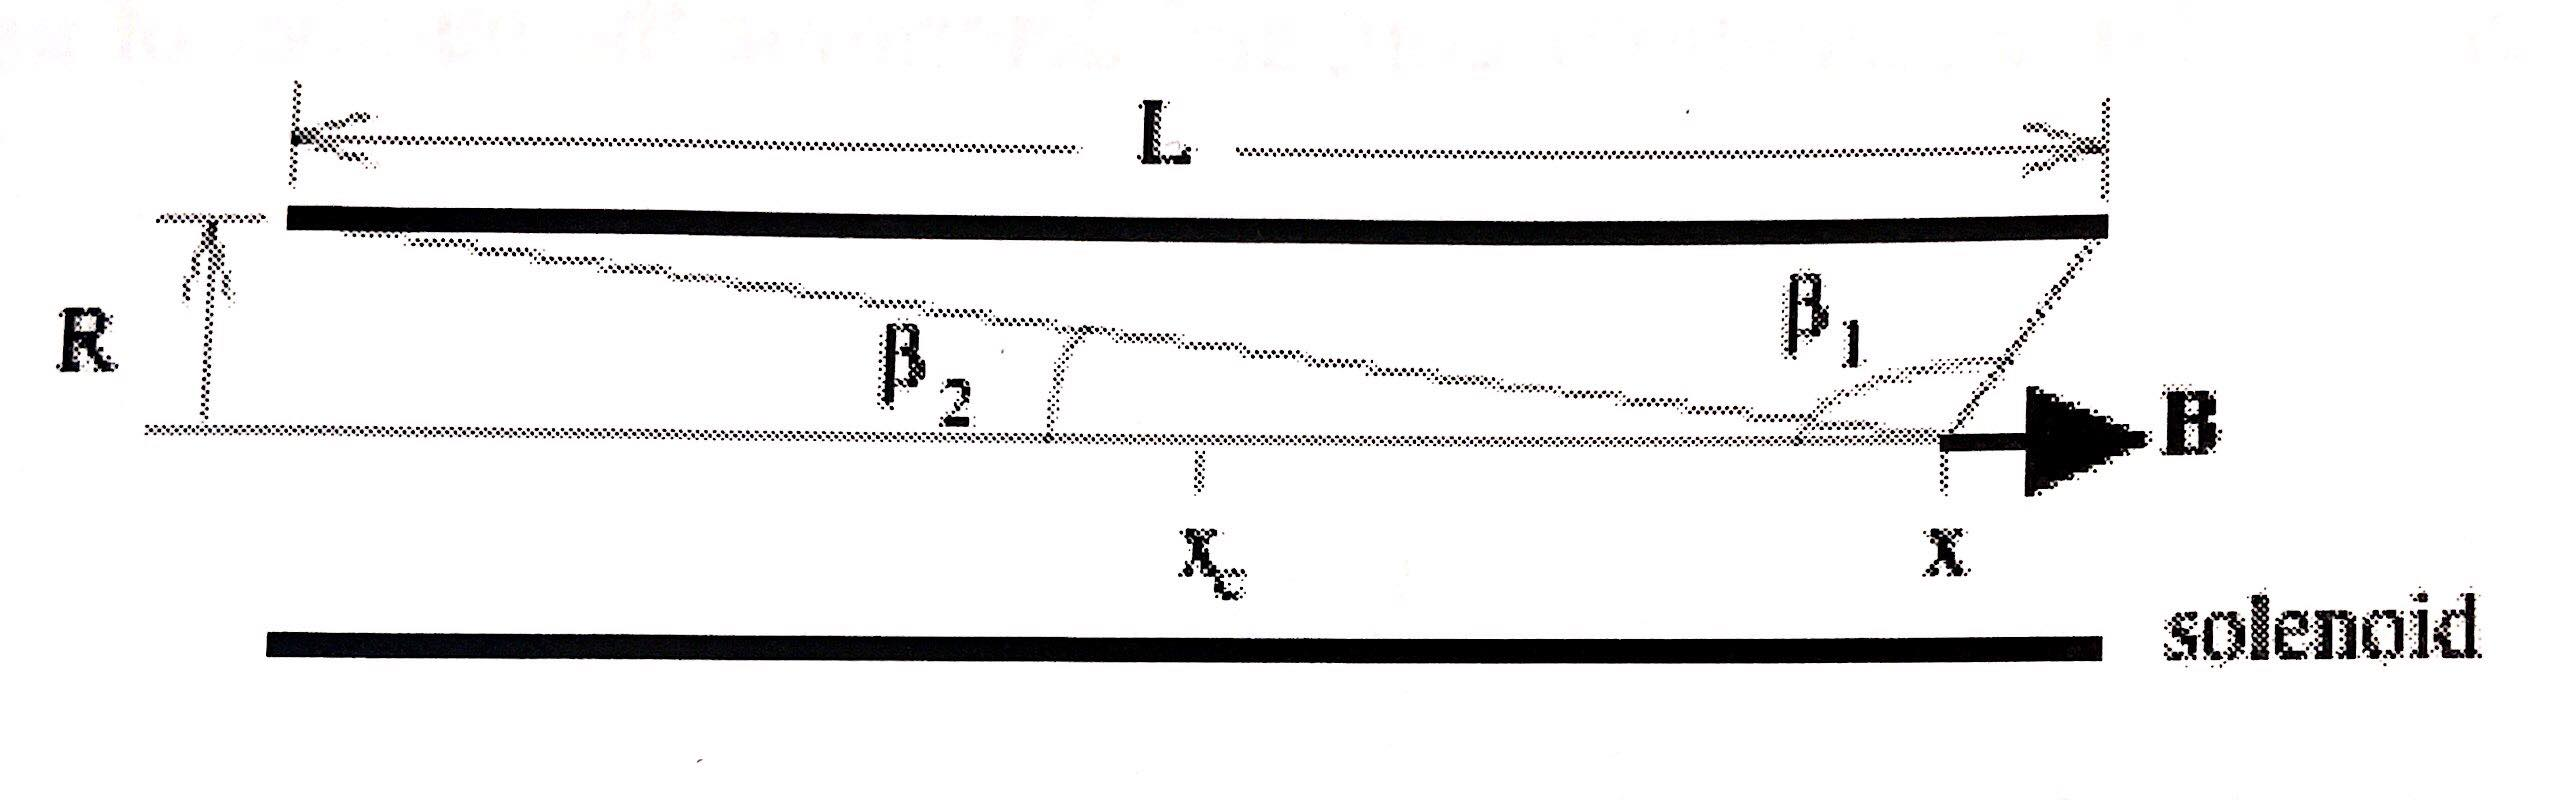
\includegraphics[width=\textwidth]{equation.jpg}
    \caption{Solenoid geometry \cite{labmanual}}
\end{figure}

We also measure the magnetic field of a Helmholtz coil, from which we experimentally determine the
number of turns of the wire in the coil using the following equations and by plotting a graph.
\begin{equation}
  B_c=\frac{\frac{1}{2}\mu_0NR^2I}{(R^2+(x-x_c)^2)^{\frac{3}{2}}}
\end{equation}
where $N$ is the number of turns, $R$ is the coil radius, $I$ is the current,
$x$ is the position along the central axis, and $x_c$ is the center position of the coil.
In our setup, we have two identical coils with the same centre axis, separated by a
distance equivalent to radius $R$. This arrangement is called a Helmholtz coil,
and the magnetic field along the axis halfway between the fields is given by:
\begin{equation}
  B_H=\frac{8\mu_0NI}{\sqrt{125}R}
\end{equation}
where $B_H$ is the magnitude of the Helmholtz magnetic field.
From the above equations, we also obtain
expressions for $B_c$, the magnetic field in the center of a single coil, and
a simplified expression for $B_s$, in the center of a real solenoid.

\section{Experimental Method}
% List all equipment used\\
% ○ Provide parameters as detailed as
% possible: masses, frequencies,
% etc.\\
% Report what YOU DID to achieve
% experimental goals:\\
% ○ Do not use imperative clause\\
% ○ Use first person narrative or
% passive voice\\
% Based on this section you should be
% able to reproduce your results without a
% manual

%use p1-2 and p2-3 to show setup


\textbf{List of Equipment:}
\begin{itemize}
  \item Solenoid Coil
  \item Helmholtz Coil
  \item DC Power Supply with variable current
  \item Switch
  \item Banana Plug Wires
  \item Hall Probe apparatus with LoggerPro software
\end{itemize}

\subsection{Part 1}

\begin{figure}[H]
    \centering
    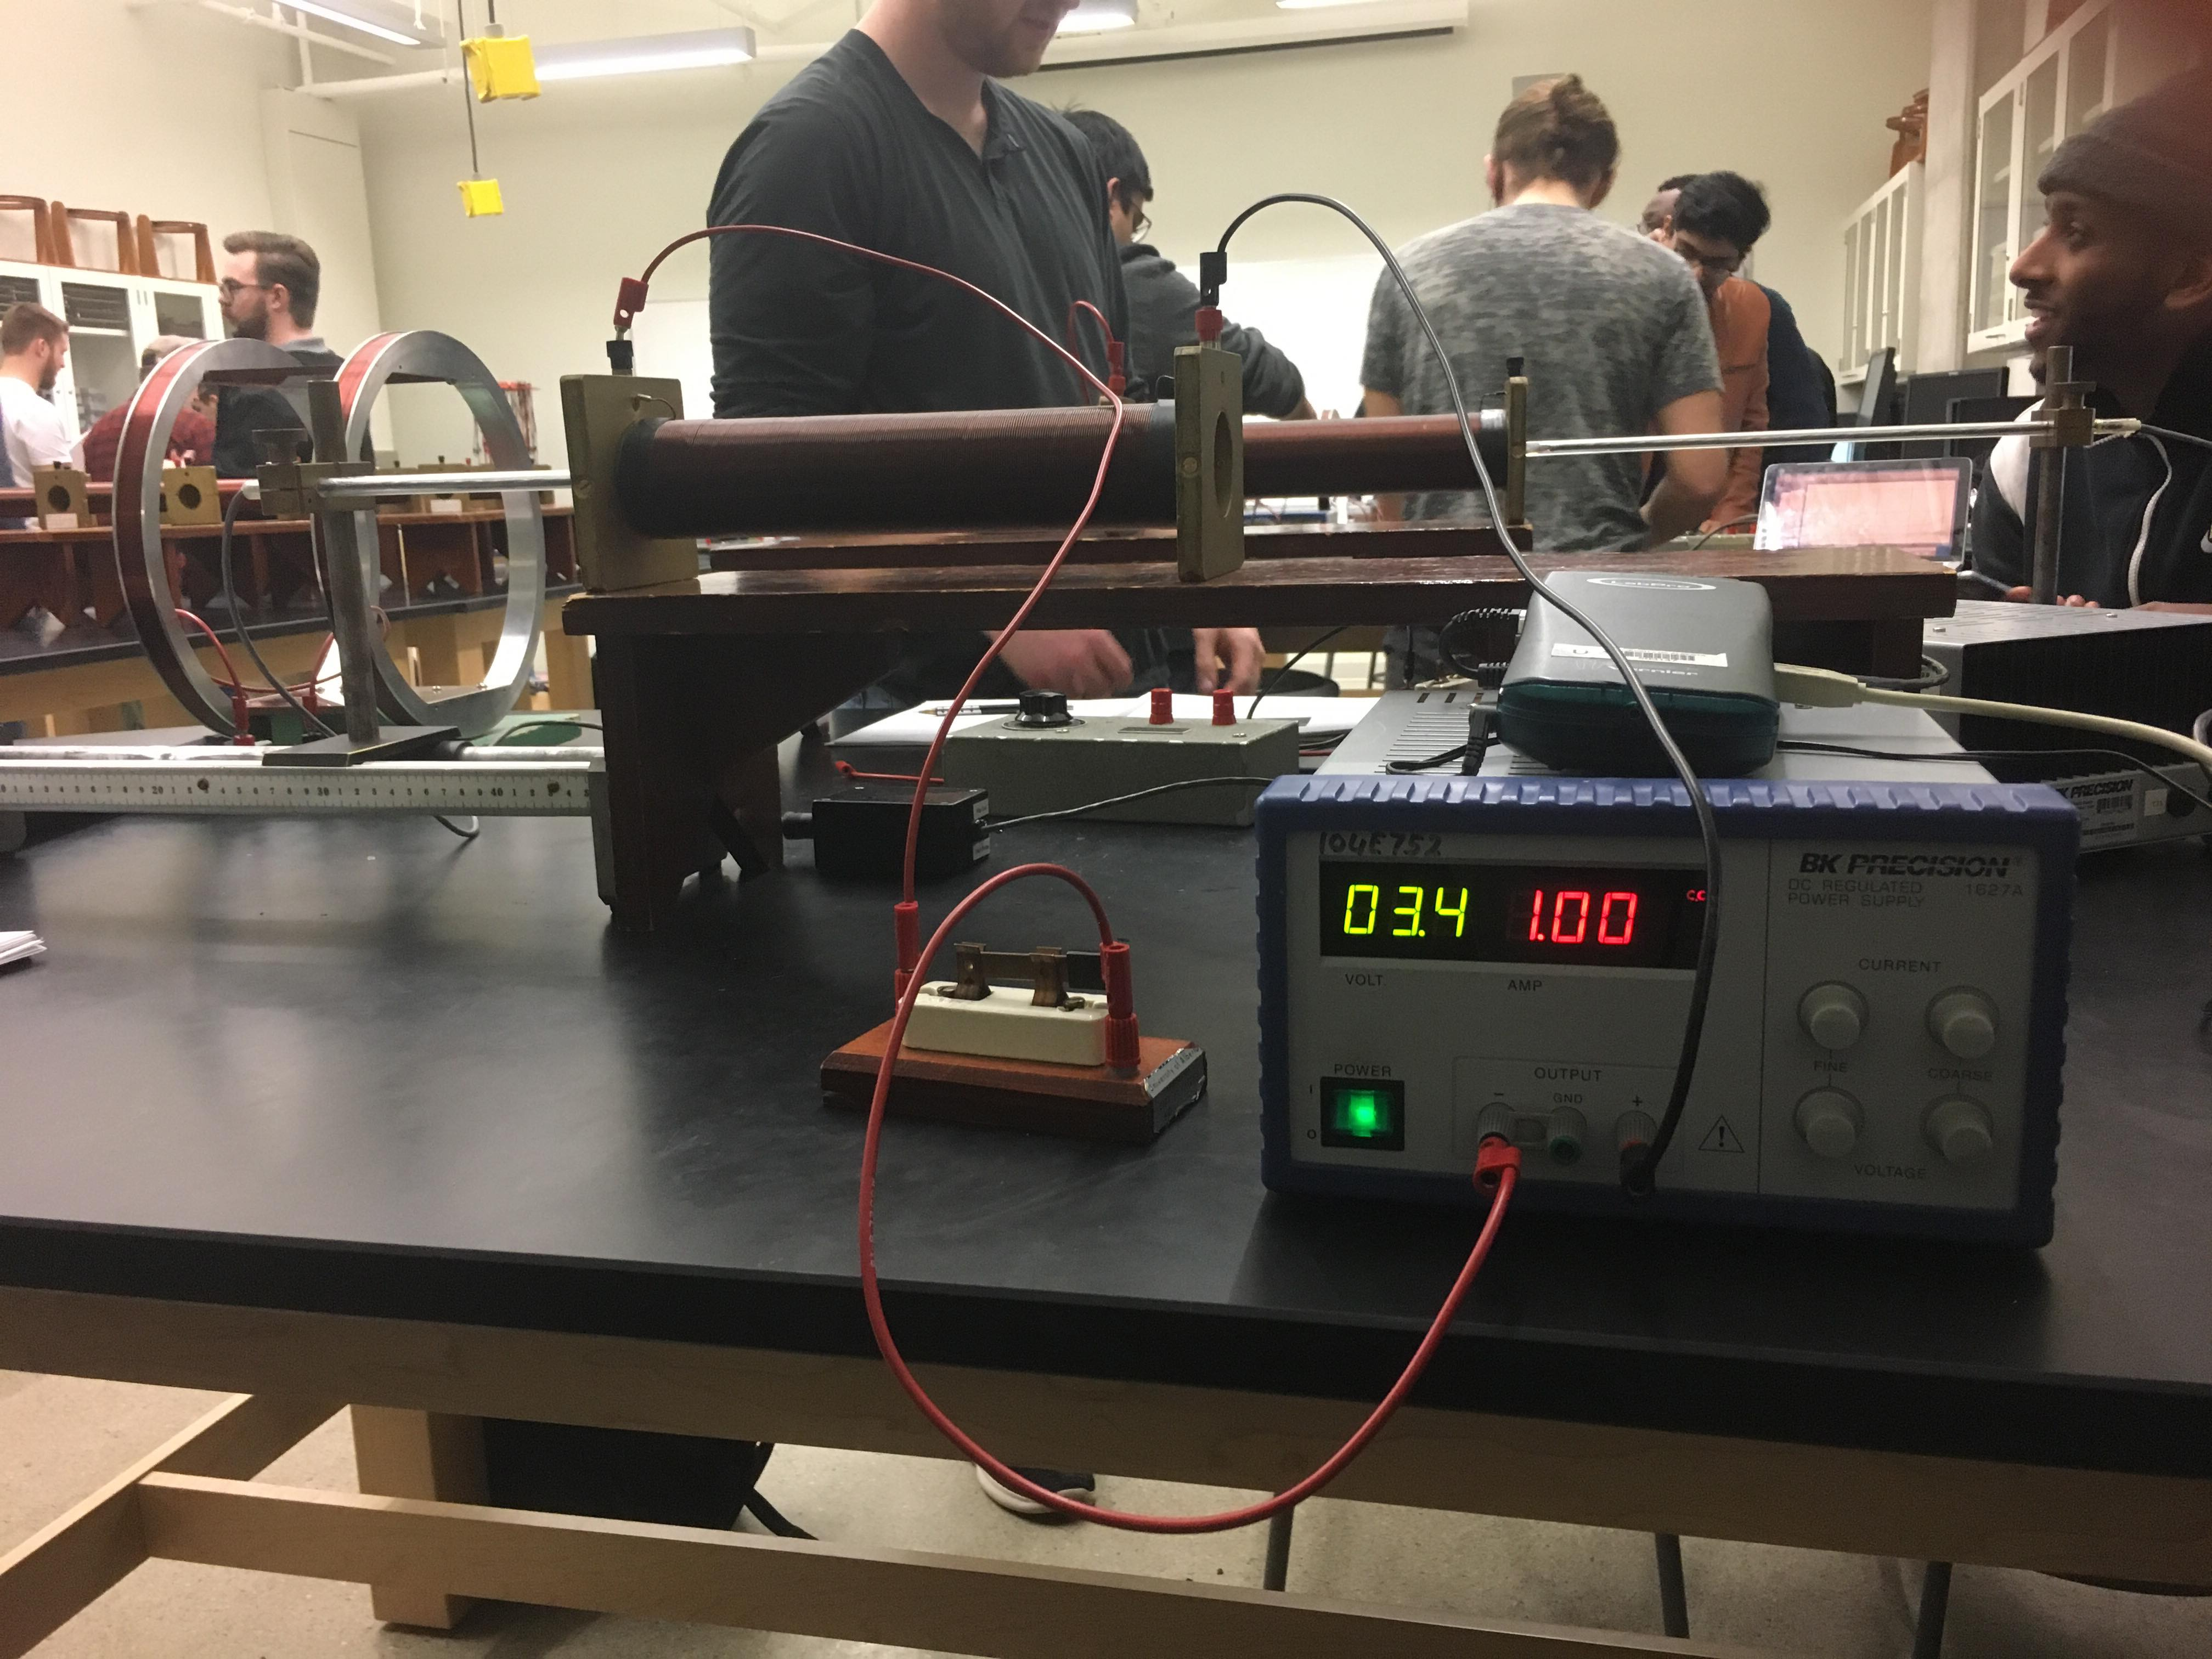
\includegraphics[width=.6\textwidth]{p1-1.jpg}
    \caption{Measuring the magnetic field of a solenoid.}
\end{figure}

The solenoid is wired as shown in Figure 2. Before the circuit is wired up,
$B_E$ is measured using the Hall apparatus. Next, the operating current in the solenoid
was set by setting the current of the power supply to $1.00 A$ with the switch closed.
If a negative value was read for the magnetic field when the switch was
closed and the power supply was on, the current in the solenoid was reversed by switching the
positive and negative leads connected to the power supply. The Hall apparatus
was set up such that the tip of the rod would be just outside of the solenoid,
and centered. From this point, the $B$ field measured in microTeslas was measured
in two centimetre increments as the Hall probe was moved inside the coil, until the
tip of the rod just barely reached the end of the coil using LoggerPro software.
Finally, the solenoid length $L$, radius $R$, number of turns $N$, operating current $I$
and ruler position $x_c$ were recorded, and the data was plotted using Excel.

\subsection{Part 2}

\begin{figure}[H]
    \centering
    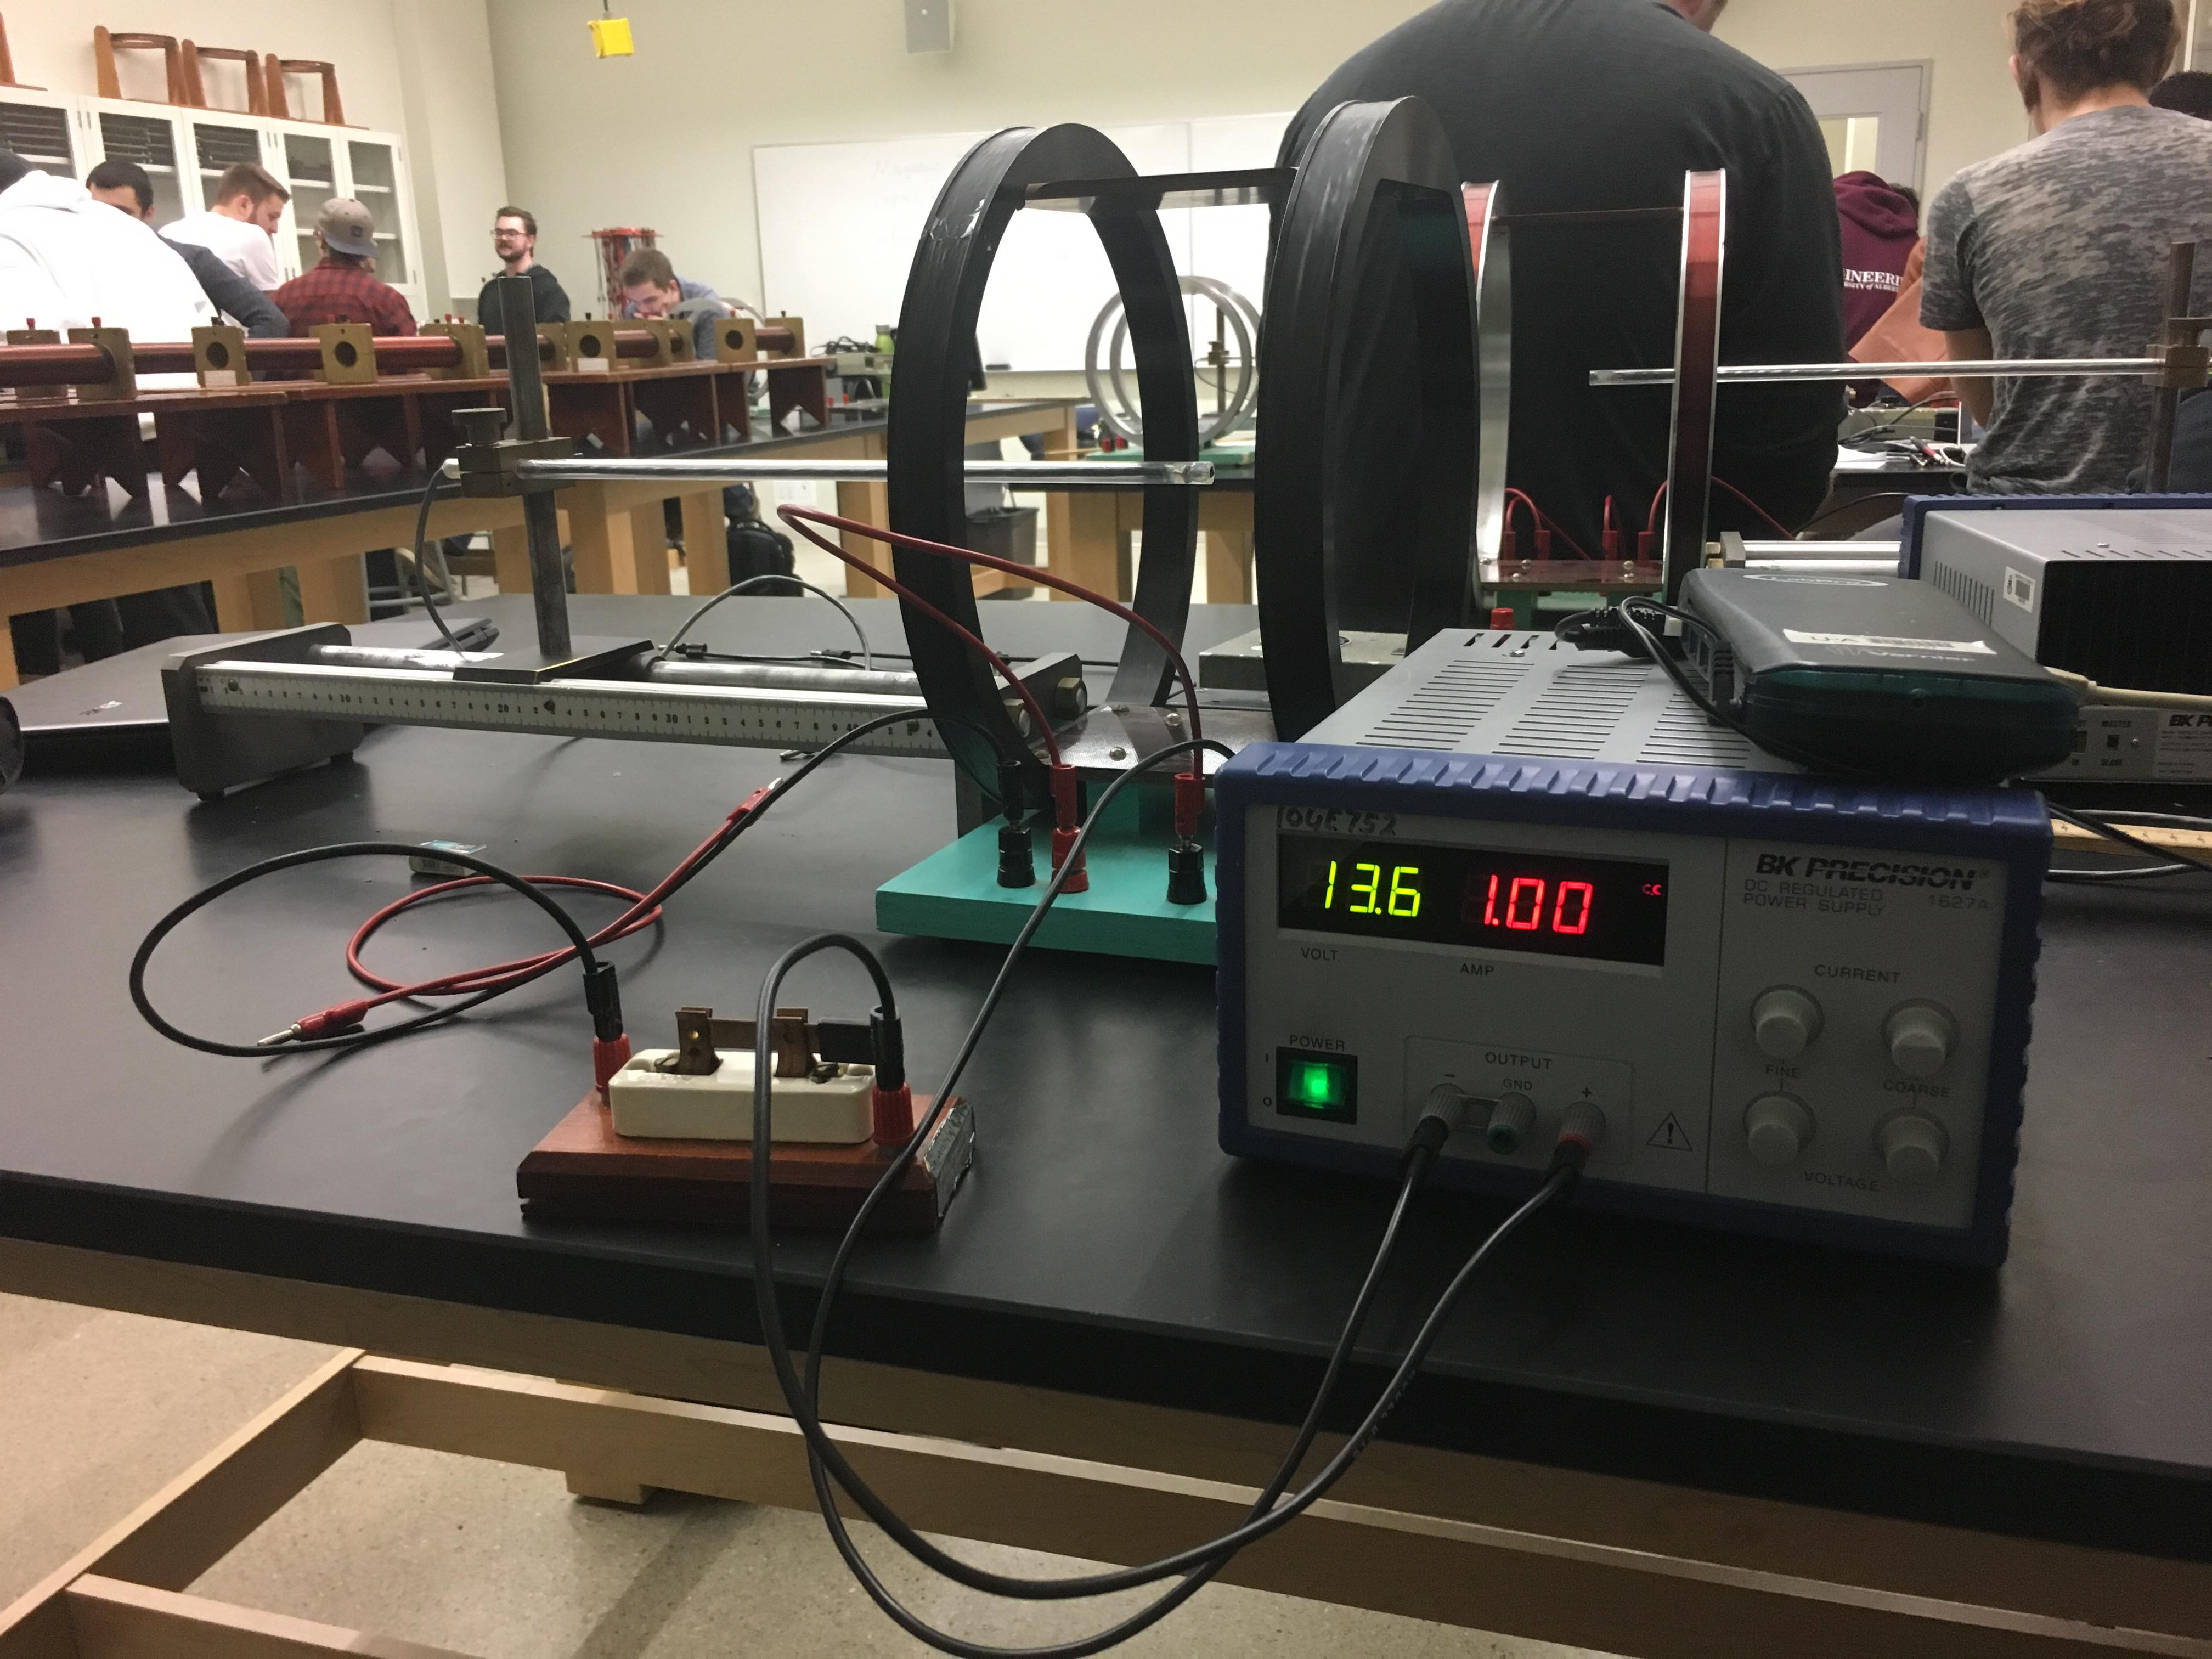
\includegraphics[width=.6\textwidth]{p2-3.jpg}
    \caption{Measuring the magnetic field of the Helmholtz coil.}
\end{figure}
The Helmholtz coils are wired as shown in Figure 3. The tip of the Hall probe
was positioned to be in the exact center of the two coils. Starting at a current
of $0.10 A$, we measured $B_H$ as the current was incremented by $0.1 A$ until
we reached a final current of $1A$. The data was recorded using LoggerPro, and
a graph was generated in Excel.


\section{Results}

\subsection{Part 1}

The constants measured and values calculated used to generate Table 2 are
as follows:

\begin{table}[H]
\centering
\begin{tabular}{ll}
Experimental Constants: & Calculated Constants:     \\ \hline
                        &                           \\
$L =0.280 \pm 0.001m$             & $\mu_0 =\SI{4 \pi e-7}{\tesla \metre \per \ampere}$   \\
$R =0.0269 \pm 0.003m$            & $\mu_0 N I/2/L = \SI{1.70E-03}{\tesla}$ \\
$N = 758$               & $R^2 =0.000724m^2$        \\
$I =1A$                 & $x_c - L/2 =0.111m$       \\
$x_c = 0.2505m$          & $x_c + L/2 = 0.391m$      \\
$B_e = -0.257mT$        &                           \\
\end{tabular}
\caption{Experimental and calculated constants}
\end{table}

Table 2 contains the measured values of the magnetic field at verious
positions in the solenoid, as well as calculated theoretical values.

\begin{table}[]
\centering
\begin{tabular}{|c|c|c|c|}
\hline
Measured B (mT) & x (m) & Corrected  $(B - B_E),\pm 2\%$ (T) & Theory $B_t$ \\ \hline
0.50            & 0.099 & 7.57E-04                           & 1.03E-03     \\ \hline
1.40            & 0.119 & 1.65E-03                           & 2.21E-03     \\ \hline
1.99            & 0.139 & 2.25E-03                           & 2.93E-03     \\ \hline
2.19            & 0.159 & 2.45E-03                           & 3.18E-03     \\ \hline
2.26            & 0.179 & 2.52E-03                           & 3.27E-03     \\ \hline
2.27            & 0.199 & 2.53E-03                           & 3.31E-03     \\ \hline
2.25            & 0.219 & 2.51E-03                           & 3.33E-03     \\ \hline
2.25            & 0.239 & 2.50E-03                           & 3.34E-03     \\ \hline
2.25            & 0.259 & 2.51E-03                           & 3.34E-03     \\ \hline
2.26            & 0.279 & 2.52E-03                           & 3.33E-03     \\ \hline
2.25            & 0.299 & 2.51E-03                           & 3.32E-03     \\ \hline
2.23            & 0.319 & 2.48E-03                           & 3.28E-03     \\ \hline
2.18            & 0.339 & 2.44E-03                           & 3.20E-03     \\ \hline
2.02            & 0.359 & 2.28E-03                           & 2.98E-03     \\ \hline
1.56            & 0.379 & 1.82E-03                           & 2.36E-03     \\ \hline
0.65            & 0.399 & 9.11E-04                           & 1.18E-03     \\ \hline
\end{tabular}
\caption{Raw data recorded while measuring $B_s$ as the Hall probe was moved in 2 centimetre increments.}
\end{table}

Using the data in Table 2, a graph is generated (Figure 4), such that we can compare our
experimental data to a theoretical curve. A sample calculation for the corrected $B-B_E$
is as follows:
$$ B-B_E = 0.5 mT - (-0.257 mT) = 0.757 mT = \SI{7.57e-4}{\tesla}$$
The theoretical $B_t$ was calculated using the Excel template downloaded from eclass.

By inspection of Figure 4 and Table 2, the ratio $\frac{B_t}{B_{exp}}$ can
be calculated, which is used to scale the slope found in Part 2 of the experiment,
which in turn is used to determine the experimental value of $N$, the number of turns in the coil.
$\frac{B_t}{B_{exp}}$ is found by picking two data points in the centre of the plateau:
$${Theoretical: } (0.259, \num{3.43e-3})$$
$${Experimental: } (0.259, \num{2.51e-3})$$
$$\therefore \frac{B_t}{B_{exp}}= \frac{\num{3.43e-3}}{\num{2.51e-3}}=1.33$$
\begin{figure}[H]
    \centering
    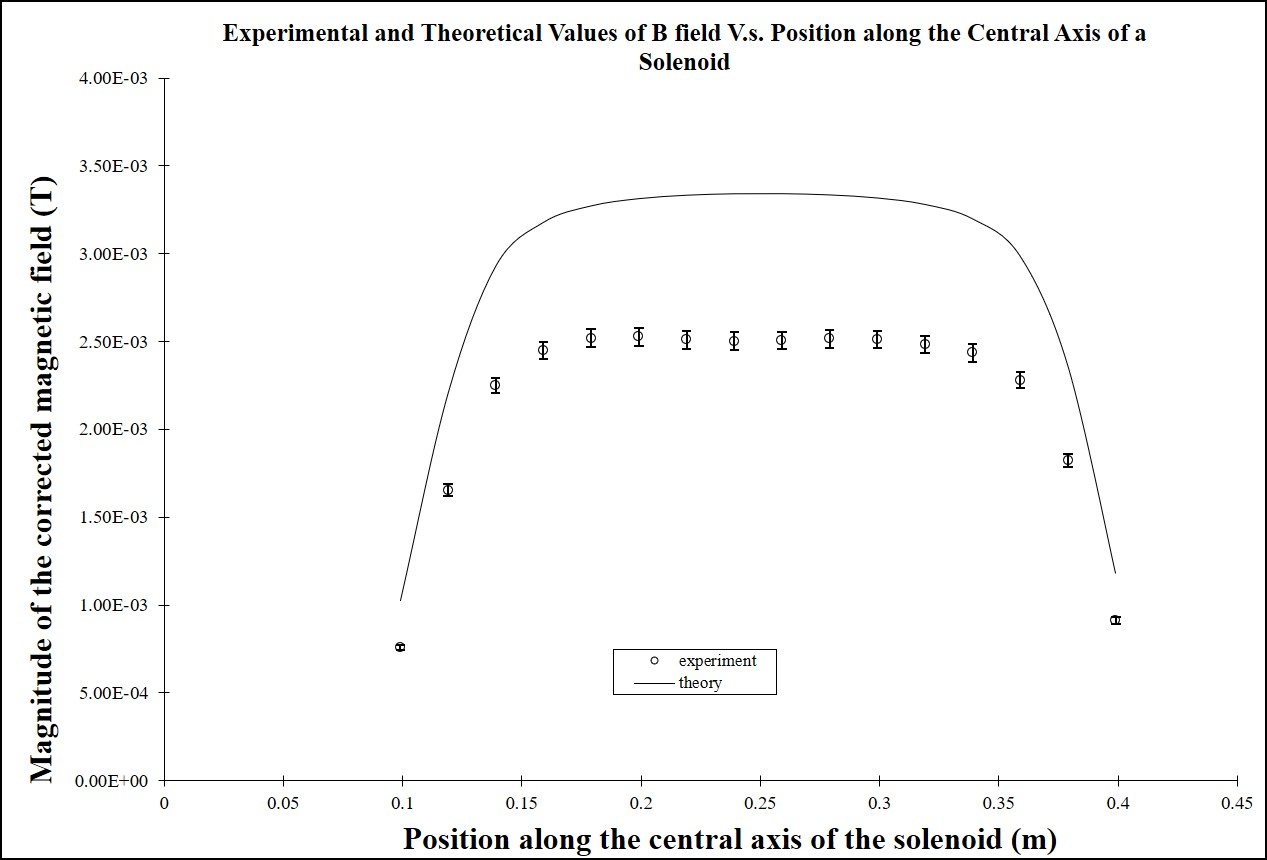
\includegraphics[width=\textwidth]{part1graph.jpg}
    \caption{Experimental values of B field in solenoid compared to theoretical values}
\end{figure}


\subsection{Part 2}

The raw data recorded for part 2 where we beasure $B_H$ in the
Helmholtz coils as a function of current is outlined in Table 2.

\begin{table}[H]
\centering
\begin{tabular}{|c|c|}
\hline
Current (A) & $B_H (T)$          \\ \hline
0.1                               & -0.000194861519119 \\ \hline
0.2                               & -0.000133962572081 \\ \hline
0.3                               & -6.99808991888E-05 \\ \hline
0.4                               & -1.21344552038E-05 \\ \hline
0.5                               & 4.36568382113E-05  \\ \hline
0.6                               & 0.000108031407536  \\ \hline
0.7                               & 0.000168628126549  \\ \hline
0.8                               & 0.000230010638426  \\ \hline
0.9                               & 0.000286799284324  \\ \hline
1                                 & 0.000351052962439  \\ \hline
\end{tabular}
\caption{Measured magnitudes of $B_H$ when varying the current in the coil in 0.1A increments}
\end{table}

Given that $R=14.8 \pm 0.2 cm$, we can linearize Equation 3 to
generate a graph (Figure 5), from which we can determine the experimental
value for N  as follows:

$$ B_H = \frac{8\mu_0NI}{\sqrt{125}R} \Rightarrow B_H = N\left( \frac{8\mu_0I}{\sqrt{125}R} \right)  $$
% $$ \therefore B_H = \frac{8 \times \SI{4 \pi e-7}{\tesla\metre\per\ampere}}{\sqrt{125}(\SI{14.8}{\cm})}$$
% $$ \Rightarrow N = \frac{B_H \sqrt{125} R}{8\mu_0I} $$
% $$ \therefore N= \frac{}{} $$
%  so we generate a graph
% with $\frac{\sqrt{2V}}{r}$ on the X axis using our measured voltage values, and $B_H$ on the Y axis
% using our measured current values.
Using the form above, we can plot a graph, such that
$B_H$ is on the y-axis, and $\frac{8\mu_0NI}{\sqrt{125}R}$ is plotted on the x-axis.
Then, our experimental value for N will be the slope, and the y-intercept should theoretically be zero.
\begin{figure}[H]
  \centering
  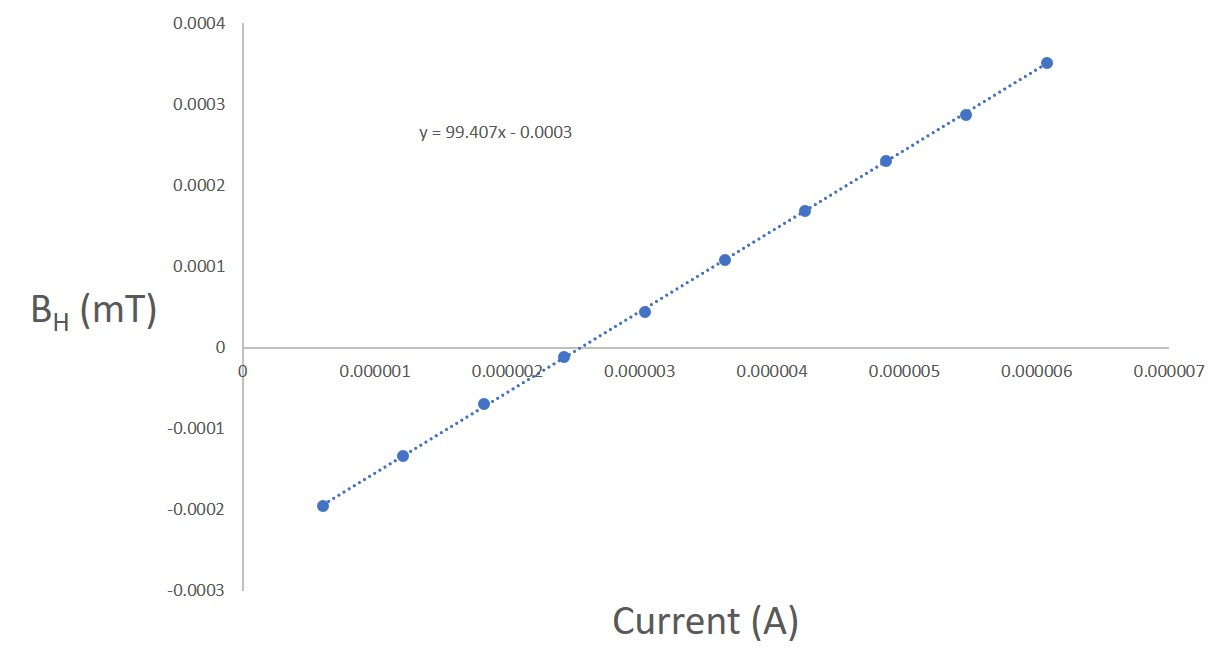
\includegraphics[width=\textwidth]{p2graph.jpg}
  \caption{$B_H$ as a function of current}
\end{figure}

\newpage
\noindent Using Excel's LINEST function, we obtain the following data from the graph in Figure 5.
\begin{table}[H]
\centering
\begin{tabular}{cc}
  Slope &  $=99.4073706 \pm 0.3873961 $ \\
        &  $=99.4 \pm 0.4$
  % Y-Intercept: &  $\num{3.99642631798173E-05}\pm \num{6.40167504007098E-06}$ \\
\end{tabular}
% \caption{LINEST data from the graph in Figure 3}
\end{table}

Now, our slope corresponds to N, however to determine our experimental
value for N, we use the scaling factor $\frac{B_t}{B_{exp}}=1.33$ which was
determined in Part 1 of the experiment.

$$ N= 99.4 \times 1.33 \approx 132 turns $$
$$ \delta N   = 0.4 \times 1.33 \approx 1 $$
$$ \therefore N = 132 \pm 1 turns$$
The theoretical $N=133$
% Now do your error calculations and theoretical value shit here.
% \noindent To obtain the calculated value for $e/m$, we can see from our LINEST data (Table 2) that the slope, $\sqrt{m/e}$ is
% $\num{2.4267255938411E-06}$.\\
% Thus, the calculated value of $e/m$ can be found:
% $$ \frac{e}{m} = \left(\sqrt{\frac{m}{e}}\right)^{-2} = 1.69808200223924714236 \times 10^{11} $$
% And the error $\delta \frac{e}{m}$ can be calculated using partial derivatives:
% $$slope= \left(\frac{e}{m}\right)^{-1/2}$$
% $$\delta slope = \left| -\frac{1}{2} \left(\frac{e}{m}\right)^{-3/2} \delta \left(\frac{e}{m}\right)\right|$$
% $$ 2 \times \delta slope = \left(\frac{e}{m}\right)^{-3/2} \delta \left(\frac{e}{m}\right) $$
% $$ \therefore \delta \left(\frac{e}{m}\right) = 2 \times \delta slope \left(\frac{e}{m}\right)^{3/2}$$
% From our LINEST data (Table 2), we know that $\delta slope = \num{3.50649774570897E-08} $
% $$ \therefore \delta \left(\frac{e}{m}\right) = 2 \times \num{3.50649774570897E-08} \times (\num{1.69808200223924714236e11})^{3/2}$$
% $$= \num{4.90728801640585e9} \approx \num{4.91e9}$$
% Thus, the calculated value for $\frac{e}{m}$ is:\footnote{Value rounded to three significant digits simply for neatness. Otherwise, the full values were messy and long}
% $$\frac{e}{m}=\num{1.70e11} \pm \SI{4.91e9}{\coulomb\per\kilogram}$$
% The percent error is:
% $$ \frac{|\num{1.69808200223924714236e11}-\num{1.76e11}|}{\num{1.76e11}}\times100 = 3.52\%$$
% Obtaining the calculated value and error for $B_E$ is a much simpler matter. We simply
% look at the data generated by LINEST, specifically, the Y-intercept (Table 2).
% $$B_E = \num{4.00E-05}\pm \SI{6.40E-06}{\tesla}$$
% The percent error is:
% $$ \frac{|\num{3.99642631798173E-05}-\num{4.8e-5}|}{\num{4.8e-5}}\times100 = 16.74\%$$

% \vspace{1cm}
% \noindent The calculated values of $e/m$ and $B_E$ from the graph are summarized in Table 3.
% \begin{table}[H]
% \centering
% \begin{tabular}{c|c|c|c|}
%                 & Expected                      & Calculated:                                     & \% Error \\ \hline
% $e/m$: & $\SI{1.76e11}{\coulomb\per\kilogram}$      & $\num{1.70e11} \pm \SI{4.91e9}{\coulomb\per\kilogram}$  &    $3.52$  \\ \hline
% $B_E$: & $4.8 \pm \,\SI{0.3e-5}{\tesla}$           & $\num{4.00e-5} \pm \,\SI{6.40e-6}{\tesla}$                    &   $16.74$  \\ \hline
% \end{tabular}
% \caption{Measured values of $e/m$ and $B_E$ compared to the calculated values obtained from the graph.}
% \end{table}

\section{Discussion}

\subsection{Part 1}

The right hand rule is used to determine the
direction of the magnetic $\textbf{B}$ field in the coils of wire. In the case of the
solenoid, the magnetic field is illustrated in Figure 5 below:

\begin{figure}[H]
    \centering
    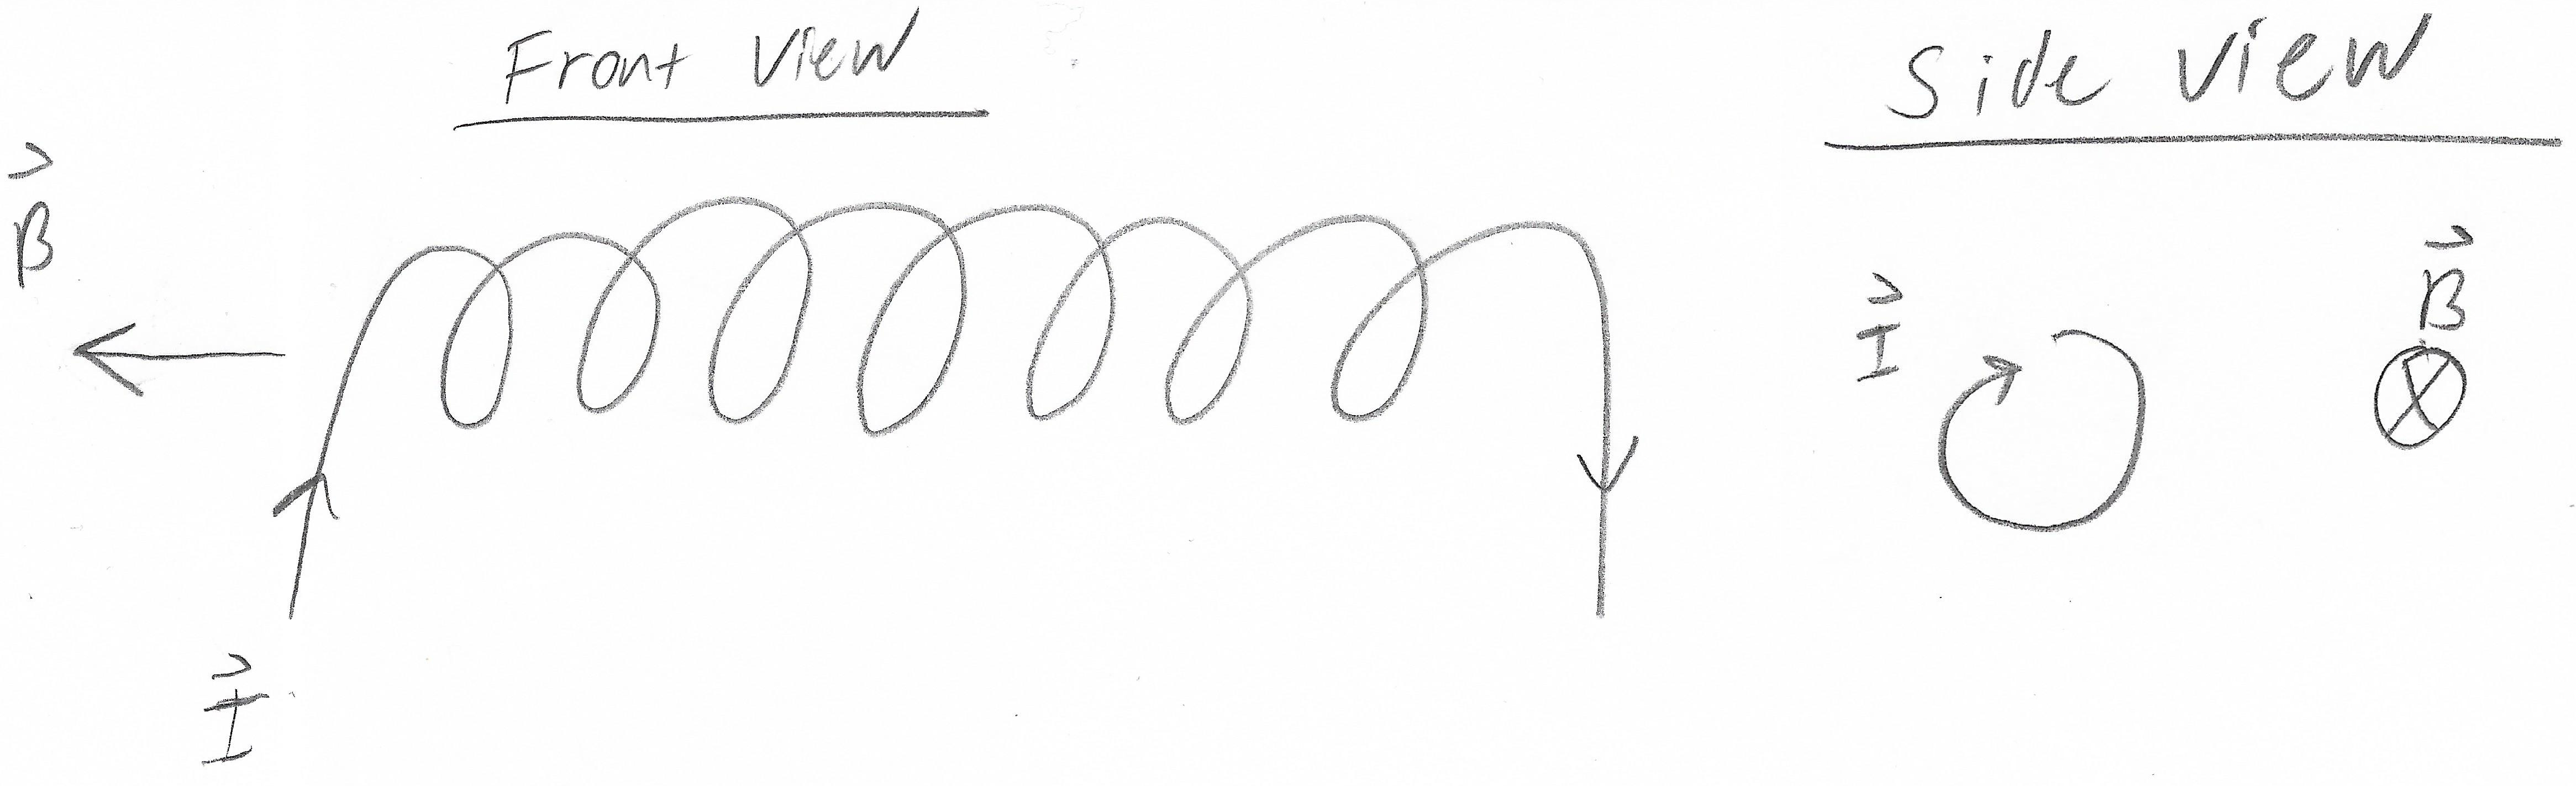
\includegraphics[width=\textwidth]{question1.jpg}
    \caption{Orientation of \textbf{B} vector for a solenoid with current \textbf{I} running through it.}
\end{figure}

From Figure 4, we can see that the experimental values measured are quite different
compared to the theoretical values. However, the shape of both curves are very similar.
In fact, if the experimental values were offset by a scaling factor $\frac{B_t}{B_{exp}=1.33}$ , our
measured results would be extremely close to the expected theoretical curve. Therefore,
the cause of error is constant, which implies that the Hall probe is likely miscalibrated,
or it could be a result of our equations not taking into account the internal resistance of the wires.



\subsection{Part 2}


The graph produced (Figure 5) is linear as expected, and looks fucking amazing.

% \begin{figure}[H]
%   \centering
%   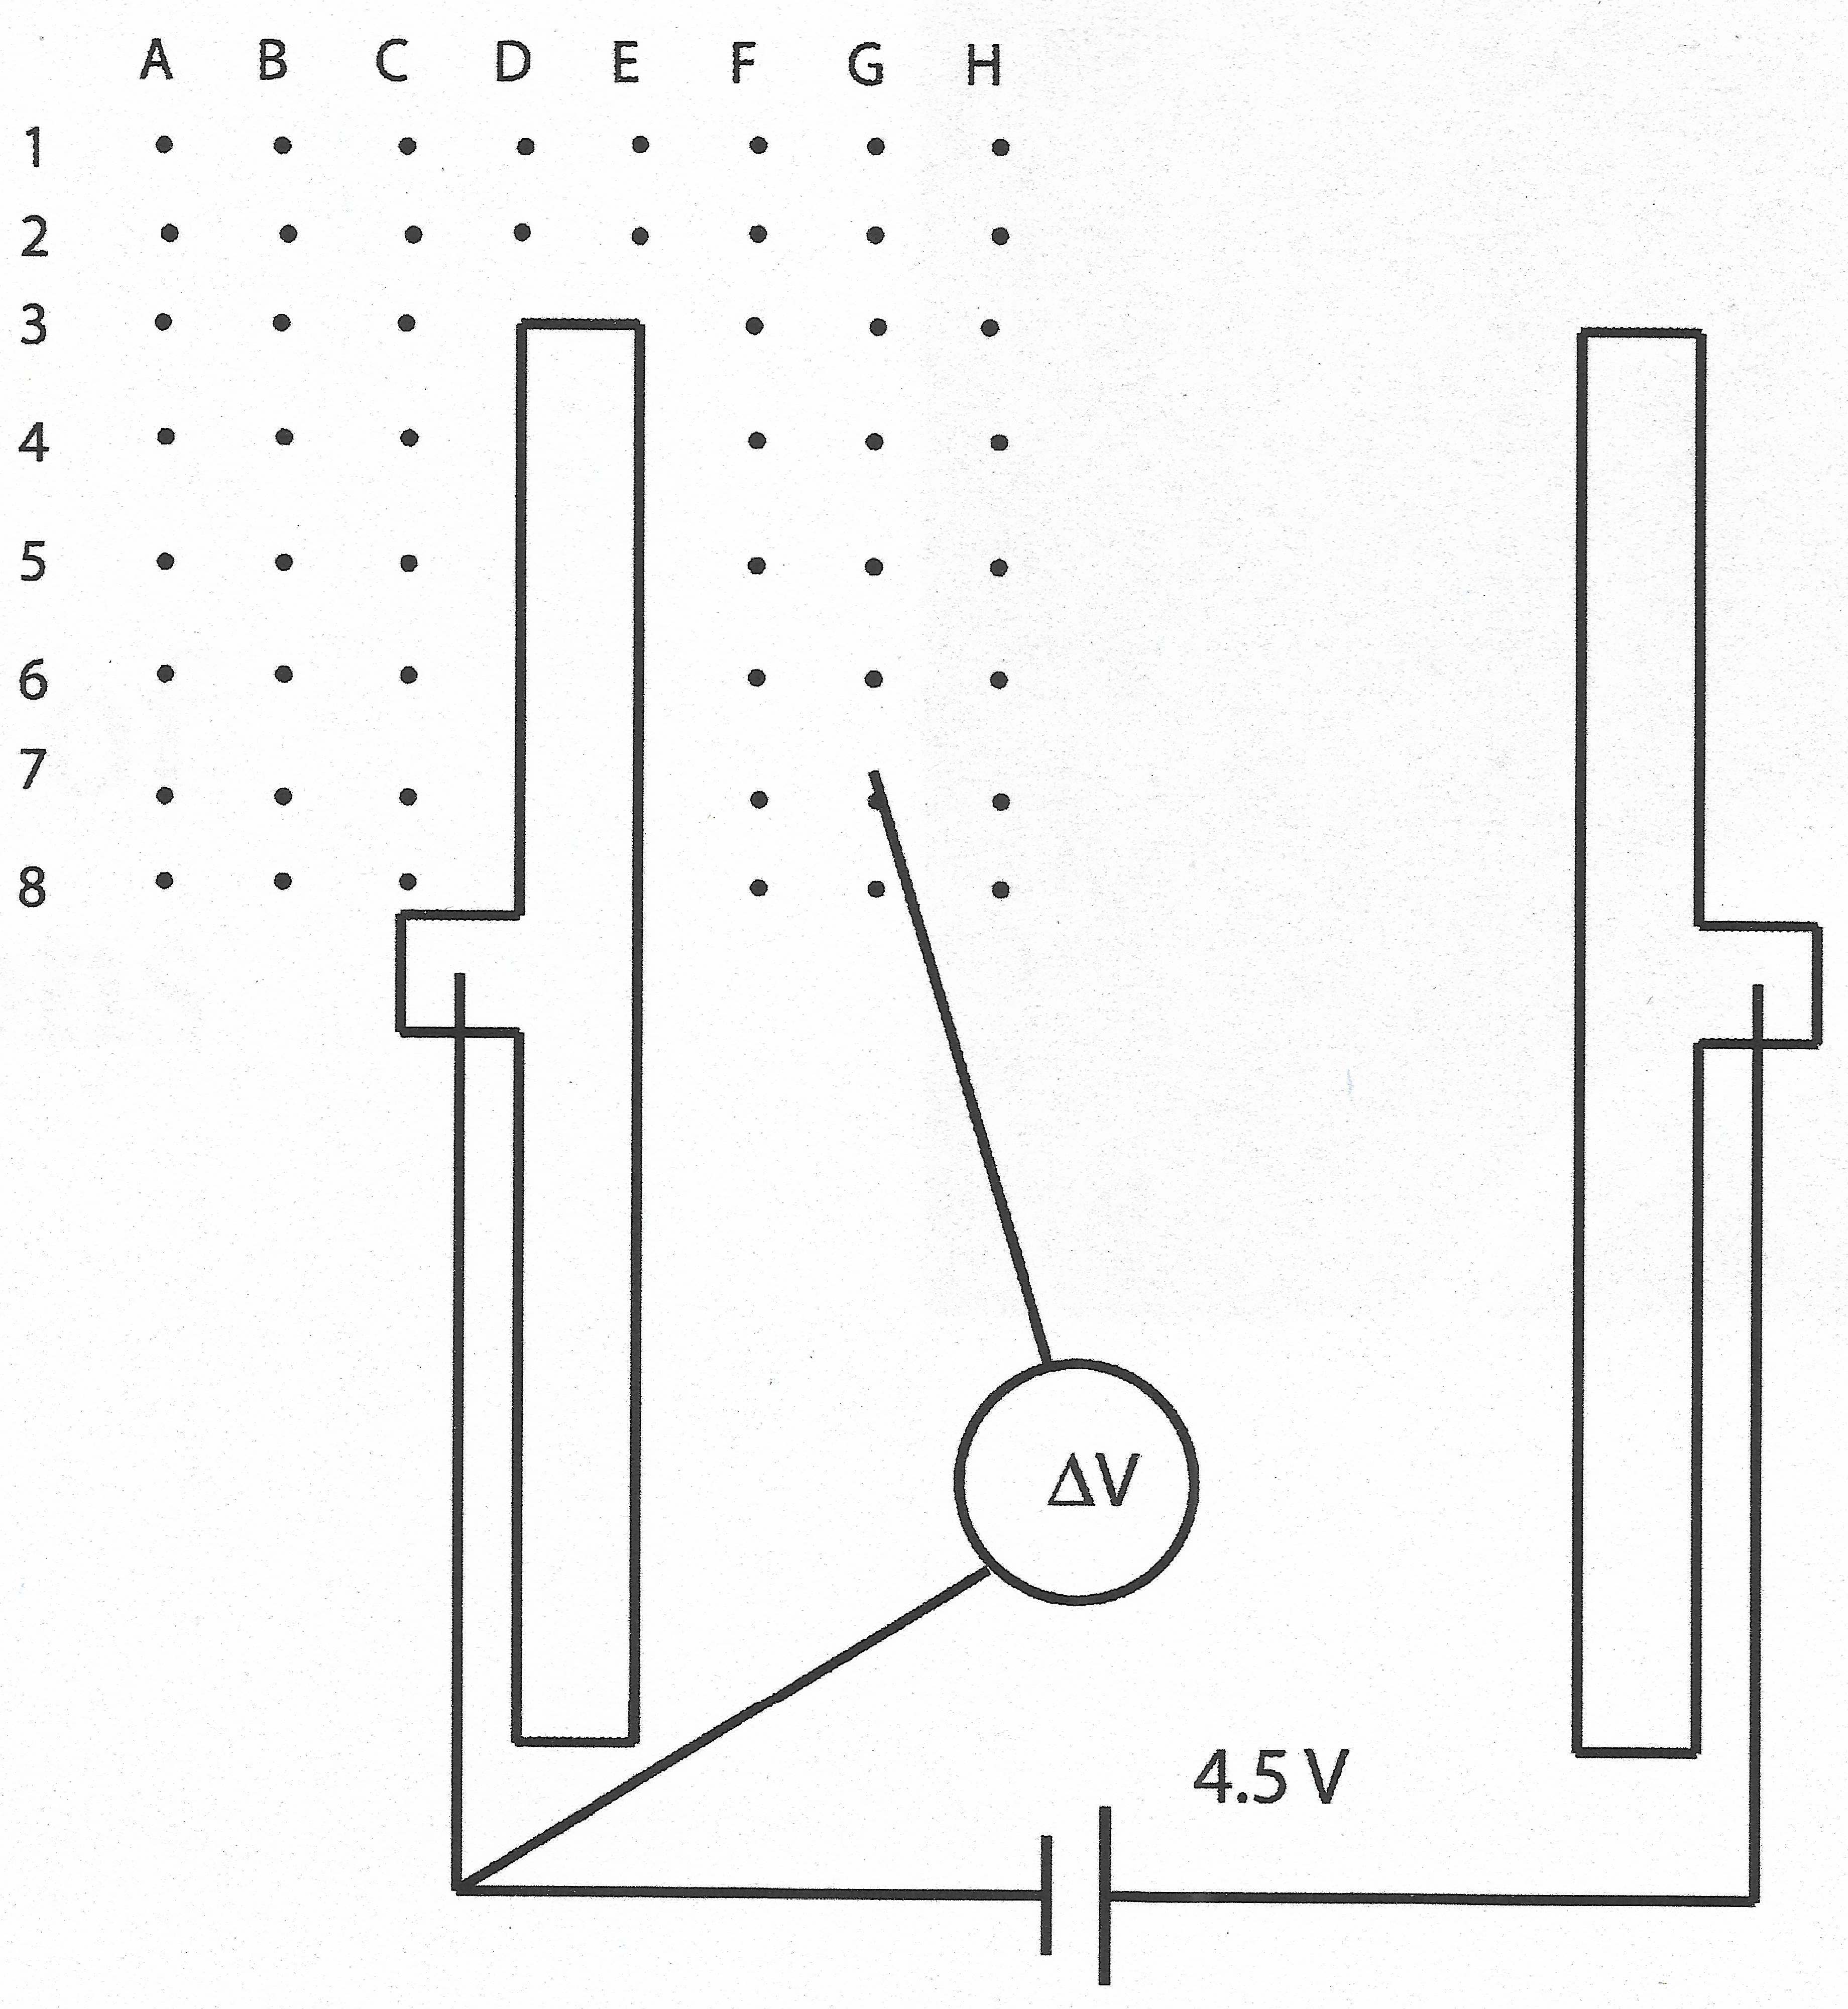
\includegraphics[width=\textwidth]{fig3.jpg}
%   \caption{The direction of the \textbf{B} field is found to be pointing out of the page when drawn this way.}
% \end{figure}

 % SOME MORE DERIVATIONS AS FOLLOWS:

Using equation 1, and the geometry from Figure 1, we can find a simplified expression for $B_s$ in the centre of a real solenoid as follows:
$$ \cos{\beta_2} = \frac{L/2}{\sqrt{R^2+L^2/4}}$$
$$ \cos{\beta_1} = \sin{(\pi/2 - \beta_1)} = -\sin{(\beta_1-\pi/2)} = -\frac{L/2}{\sqrt{R^2+L^2/4}}  $$
Substituting into equation 1 yields:
$$ B_s = 1/2 \mu_0nI \left(\frac{L/2}{\sqrt{R^2+L^2/4}} + \frac{L/2}{\sqrt{R^2+L^2/4}} \right) =  1/2\mu_0nI \left(\frac{L}{\sqrt{R^2+L^2/4}} \right)= \frac{\mu_0nIL}{\sqrt{4R^2+L^2}}$$
Since $n=N/L$, we can substitute $nL=N$ to finally obtain:
$$ B_s= \frac{\mu_0NI}{\sqrt{4R^2+L^2}} $$
%and compare it to the
%expected value of 133. The radius of each coil is $14.8\pm 0.2cm$

We can also find the simplified expression for $B_s$ in the centre of a real solenoid as follows:
$$1$$
Next, the expression for $B_c$ in the center of a single coil can be found:
$$2$$
Additionally, the expression for $B_H$ can be obtained from the expression for $B_c$ derived above:
$$3$$

Using the scaling factor 1.33 derived in part 1 of the experiment, we obtain the value $N=132 \pm 1$,
which agrees within error of the theoretical value 133.
\section{Conclusions}

In Experiment 2, we measure the distribution of the magnetic field across a solenoid,
and we also measure the magnetic field of a Helmholtz coil from which we experimentally determine the
number of turns of the wire in the coil. In the first part, q Hall probe was used to measure the magnetic field
at various points inside a solenoid. The graph produced from our experimental values
closely matched the shape of the theoretical curve, even though the measured values were
quite different from the theoretical values. It should be noted that if each recorded
data point was offset by some correction amount, the measured values would fit the
theoretical curve very nicely, which implies that the Hall probe
was likely miscalibrated, or some factor was not being taken into account such as the internal resistance
of the wires. In part 2, the Hall probe was used to measure the magnetic field
at the center of the Helmholtz coils with varying current, from which we could experimentally
determine the number of turns of the wire in the coils. The measured values were XXXXXXXXXXXXXXXXXXXXXXx
and compared to the theoretical XXXXXXXXXXXXXx it did / did not agree within error.
% In Experiment 3, we calculate the charge to mass ratio $e/m$ of electrons fired in a Helmholtz coil, which are accelerated by an electric field, and
% deflected by a magnetic field to form a circular orbit. The apparatus
% was set up such that the magnetic field of the coil is aligned antiparallel to the earth's own magnetic field
% to simplify the geomery. The current was varied at three diferent voltages to align the electron loops to known radii, so that we could use the
% Helmholtz curents to calculate a value for $e/m$, and the earth's magnetic field $B_E$ by ploting a linear graph. We noticed that the
% radius of curvature of the electron loops increased as the Helmholtz current was lowered. Additionally, using the
% left hand rule (since electrons are negatively charged masses), we verified that the net magnetic field of the
% setup was directed upwards, in the same orientation of the coil (in other words, the direction of the net magnetic field
% was perpendicular to the radius of the coil). We calculated the charge to mass ratio of the electron to be ($\num{1.70e11} \pm \SI{4.91e9}{\coulomb\per\kilogram}$)
% and the earth's magnetic field to be
% ($\num{4.00e-5} \pm \,\SI{6.40e-6}{\tesla}$). While these values are in the same order of magnitude as the
% expected values ( $\SI{1.76e11}{\coulomb\per\kilogram}$ for $e/m$
% and $4.8 \pm \,\SI{0.3e-5}{\tesla}$ for $B_E$), these values do not agree within error. The
% graph generated from our data was linear, however, so it is likely that the source of error introduced was a
% constant factor, whether it's miscalibration of equipment, or human error since we took care to record our
% results in a consistent manner.

\bibliography{references}
\end{document}
